\documentclass[10pt,ignorenonframetext,aspectratio=169,t,]{beamer} % aspectratio=169,t,

\setbeamertemplate{caption}[numbered]
\setbeamertemplate{caption label separator}{: }
\setbeamercolor{caption name}{fg=normal text.fg}

\beamertemplatenavigationsymbolsempty

\usepackage{lmodern}

\usepackage{amssymb,amsmath}
\usepackage{ifxetex,ifluatex}
\usepackage{fixltx2e} % provides \textsubscript
\ifnum 0\ifxetex 1\fi\ifluatex 1\fi=0 % if pdftex
  \usepackage[T1]{fontenc}
  \usepackage[utf8]{inputenc}

\else % if luatex or xelatex
  \ifxetex
    \usepackage{mathspec}
  \else
    \usepackage{fontspec}
  \fi
  \defaultfontfeatures{Ligatures=TeX,Scale=MatchLowercase}

\fi


% use upquote if available, for straight quotes in verbatim environments
\IfFileExists{upquote.sty}{\usepackage{upquote}}{}
% use microtype if available
\IfFileExists{microtype.sty}{%
\usepackage{microtype}
\UseMicrotypeSet[protrusion]{basicmath} % disable protrusion for tt fonts
}{}

\newif\ifbibliography
\hypersetup{
            pdftitle={基于RMarkdown快速制作学术幻灯片},
            pdfauthor={魏江勇 (Jiangyong Wei)},
            pdfborder={0 0 0},
            breaklinks=true}
\urlstyle{same}  % don't use monospace font for urls
\usepackage{color}
\usepackage{fancyvrb}
\newcommand{\VerbBar}{|}
\newcommand{\VERB}{\Verb[commandchars=\\\{\}]}
\DefineVerbatimEnvironment{Highlighting}{Verbatim}{commandchars=\\\{\}}
% Add ',fontsize=\small' for more characters per line
\usepackage{framed}
\definecolor{shadecolor}{RGB}{48,48,48}
\newenvironment{Shaded}{\begin{snugshade}}{\end{snugshade}}
\newcommand{\KeywordTok}[1]{\textcolor[rgb]{0.94,0.87,0.69}{{#1}}}
\newcommand{\DataTypeTok}[1]{\textcolor[rgb]{0.87,0.87,0.75}{{#1}}}
\newcommand{\DecValTok}[1]{\textcolor[rgb]{0.86,0.86,0.80}{{#1}}}
\newcommand{\BaseNTok}[1]{\textcolor[rgb]{0.86,0.64,0.64}{{#1}}}
\newcommand{\FloatTok}[1]{\textcolor[rgb]{0.75,0.75,0.82}{{#1}}}
\newcommand{\ConstantTok}[1]{\textcolor[rgb]{0.86,0.64,0.64}{\textbf{{#1}}}}
\newcommand{\CharTok}[1]{\textcolor[rgb]{0.86,0.64,0.64}{{#1}}}
\newcommand{\SpecialCharTok}[1]{\textcolor[rgb]{0.86,0.64,0.64}{{#1}}}
\newcommand{\StringTok}[1]{\textcolor[rgb]{0.80,0.58,0.58}{{#1}}}
\newcommand{\VerbatimStringTok}[1]{\textcolor[rgb]{0.80,0.58,0.58}{{#1}}}
\newcommand{\SpecialStringTok}[1]{\textcolor[rgb]{0.80,0.58,0.58}{{#1}}}
\newcommand{\ImportTok}[1]{\textcolor[rgb]{0.80,0.80,0.80}{{#1}}}
\newcommand{\CommentTok}[1]{\textcolor[rgb]{0.50,0.62,0.50}{{#1}}}
\newcommand{\DocumentationTok}[1]{\textcolor[rgb]{0.50,0.62,0.50}{{#1}}}
\newcommand{\AnnotationTok}[1]{\textcolor[rgb]{0.50,0.62,0.50}{\textbf{{#1}}}}
\newcommand{\CommentVarTok}[1]{\textcolor[rgb]{0.50,0.62,0.50}{\textbf{{#1}}}}
\newcommand{\OtherTok}[1]{\textcolor[rgb]{0.94,0.94,0.56}{{#1}}}
\newcommand{\FunctionTok}[1]{\textcolor[rgb]{0.94,0.94,0.56}{{#1}}}
\newcommand{\VariableTok}[1]{\textcolor[rgb]{0.80,0.80,0.80}{{#1}}}
\newcommand{\ControlFlowTok}[1]{\textcolor[rgb]{0.94,0.87,0.69}{{#1}}}
\newcommand{\OperatorTok}[1]{\textcolor[rgb]{0.94,0.94,0.82}{{#1}}}
\newcommand{\BuiltInTok}[1]{\textcolor[rgb]{0.80,0.80,0.80}{{#1}}}
\newcommand{\ExtensionTok}[1]{\textcolor[rgb]{0.80,0.80,0.80}{{#1}}}
\newcommand{\PreprocessorTok}[1]{\textcolor[rgb]{1.00,0.81,0.69}{\textbf{{#1}}}}
\newcommand{\AttributeTok}[1]{\textcolor[rgb]{0.80,0.80,0.80}{{#1}}}
\newcommand{\RegionMarkerTok}[1]{\textcolor[rgb]{0.80,0.80,0.80}{{#1}}}
\newcommand{\InformationTok}[1]{\textcolor[rgb]{0.50,0.62,0.50}{\textbf{{#1}}}}
\newcommand{\WarningTok}[1]{\textcolor[rgb]{0.50,0.62,0.50}{\textbf{{#1}}}}
\newcommand{\AlertTok}[1]{\textcolor[rgb]{1.00,0.81,0.69}{{#1}}}
\newcommand{\ErrorTok}[1]{\textcolor[rgb]{0.76,0.75,0.62}{{#1}}}
\newcommand{\NormalTok}[1]{\textcolor[rgb]{0.80,0.80,0.80}{{#1}}}
\usepackage{graphicx,grffile}
\makeatletter
\def\maxwidth{\ifdim\Gin@nat@width>\linewidth\linewidth\else\Gin@nat@width\fi}
\def\maxheight{\ifdim\Gin@nat@height>\textheight0.8\textheight\else\Gin@nat@height\fi}
\makeatother
% Scale images if necessary, so that they will not overflow the page
% margins by default, and it is still possible to overwrite the defaults
% using explicit options in \includegraphics[width, height, ...]{}
\setkeys{Gin}{width=\maxwidth,height=\maxheight,keepaspectratio}

% Prevent slide breaks in the middle of a paragraph:
\widowpenalties 1 10000
\raggedbottom

\AtBeginPart{
  \let\insertpartnumber\relax
  \let\partname\relax
  \frame{\partpage}
}
\AtBeginSection{
  \ifbibliography
  \else
    \let\insertsectionnumber\relax
    \let\sectionname\relax
    \frame{\sectionpage}
  \fi
}
\AtBeginSubsection{
  \let\insertsubsectionnumber\relax
  \let\subsectionname\relax
  \frame{\subsectionpage}
}

\setlength{\parindent}{0pt}
\setlength{\parskip}{6pt plus 2pt minus 1pt}
\setlength{\emergencystretch}{3em}  % prevent overfull lines
\providecommand{\tightlist}{%
  \setlength{\itemsep}{0pt}\setlength{\parskip}{0pt}}
\setcounter{secnumdepth}{0}
\usepackage{xeCJK}
\usepackage{tikz,graphicx}    
\usepackage{booktabs}       
\usepackage[normalem]{ulem}   
\usepackage{rotating}       
\usepackage{cleveref}       
\usepackage{hyperref}       
\usepackage[absolute,overlay]{textpos}
\usepackage{xltxtra} % “Extras” for LATEX users of XETEX

\hypersetup{pdfpagemode=FullScreen}
\hypersetup{colorlinks=false}


\setbeamertemplate{navigation symbols}{} % remove navigation symbols in beamer
\setbeamertemplate{title page}[empty]    % Setting up your own title page template
\setbeamercovered{transparent}           % Transparency in itemizing

\addtobeamertemplate{title page}{
\tikz[overlay,remember picture] \node[opacity=0.3, at=(current page.center)] {
   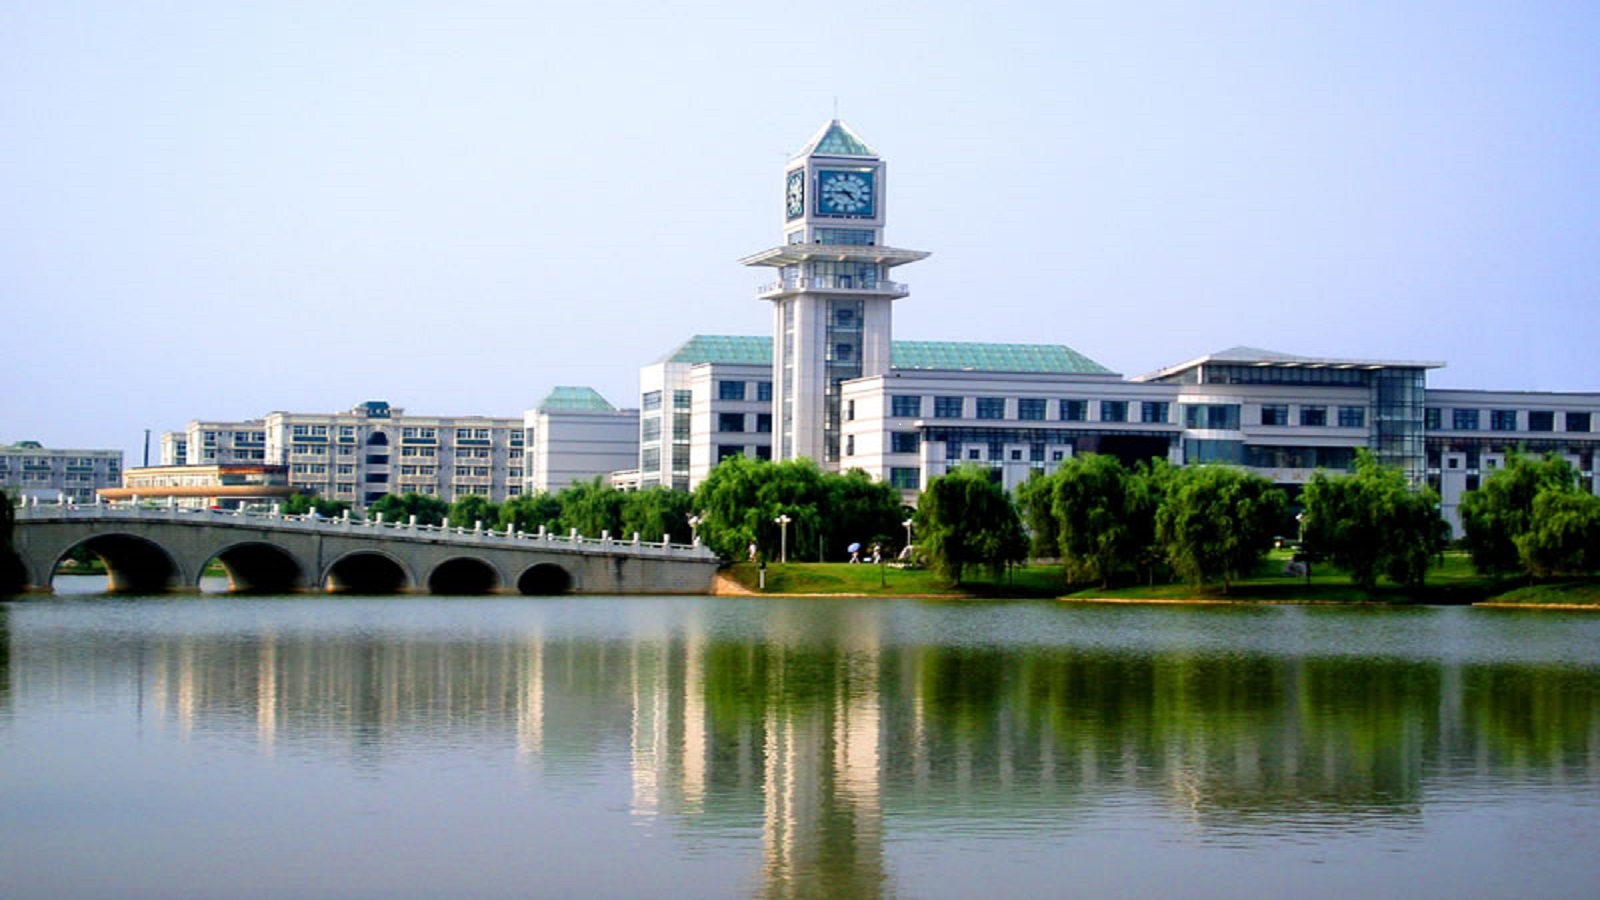
\includegraphics[width=\paperwidth,height=\paperheight,]{./figureFiles/znufebg169.jpg}};
}

%%%%%%%%%%%%%%%%%%%%%%%%%%%%%%%%%%%%%%%%%%%%%%%
% \institute{
%   {中南财经政法大学} \\
%   {\tiny 统计与数学学院} \\
%   \smallskip                                          
%   \emph {\tiny datalab026a@qq.com}                      
% }

% \institute{
%     {Zhongnan University of Economics and Law} \\
%     {\tiny School of Statistics and Mathematics} \\
%     \smallskip                                          
%     \emph {\scriptsize datalab026a@qq.com}                      
% }
%%%%%%%%%%%%%%%%%%%%%%%%%%%%%%%%%%%%%%%%%%%%%%%%%

% \usefonttheme{professionalfonts} % using non standard fonts for beamer
% \usefonttheme{serif}     % default family is serif
% \usepackage[T1]{fontenc} % Standard package for selecting font encodings
% \usepackage{lmodern}     % Latin modern fonts in outline formats

% Chinese font support

\setmainfont{Noto Serif}
\setsansfont{Noto Sans}
\setmonofont[Mapping=tex-ansi]{Noto Mono}

\setCJKmainfont{Noto Sans CJK SC}
\setCJKsansfont{Noto Sans CJK SC}
\setCJKmonofont{Noto Sans CJK SC}

\usefonttheme{default}

\setbeamerfont{title}{size=\Large,series=\bfseries,parent=structure}
\setbeamerfont{subtitle}{size=\small,series=\bfseries,parent=structure}
\setbeamerfont{section in head/foot}{size=\tiny,series=\bfseries}
\setbeamerfont{section in toc}{size=\large,series=\bfseries,parent=structure}
\setbeamerfont{frametitle}{series=\bfseries}
\setbeamerfont{author}{size=\small}
\setbeamerfont{date}{size=\scriptsize} 

\setbeamertemplate{bibliography item}[mybibitem]
\setbeamerfont{bibliography entry author}{shape=\upshape,series=\bfseries,size=\normalsize}%
\setbeamerfont{bibliography entry title}{shape=\upshape,size=\small,series=\mdseries}
\setbeamerfont{bibliography entry journal}{shape=\upshape,size=\small,series=\mdseries}
\setbeamerfont{bibliography entry note}{shape=\upshape,size=\small,series=\mdseries}

\setbeamerfont{itemize/enumerate body}{size=\small}
\setbeamerfont{itemize/enumerate subbody}{size=\footnotesize}
\setbeamerfont{itemize/enumerate subsubbody}{size=\scriptsize}

\setbeamerfont{block title}{size=\normalsize,series=\bfseries,parent={structure,block body}}



\definecolor{texpurple}{HTML}{522D80}
\definecolor{texorange}{HTML}{F66733}
\definecolor{texblue}{HTML}{2B3856}
\definecolor{antiquewhite}{rgb}{0.98, 0.92, 0.84}
\definecolor{aliceblue}{rgb}{0.94, 0.97, 1.0}
\definecolor{lighttaupe}{rgb}{0.7, 0.55, 0.43}
\definecolor{mediumtaupe}{rgb}{0.4, 0.3, 0.28}
\definecolor{taupe}{rgb}{0.28, 0.24, 0.2}
\definecolor{darktaupe}{rgb}{0.28, 0.24, 0.2}
\definecolor{camouflagegreen}{rgb}{0.47, 0.53, 0.42}

% \setbeamercolor{frametitle}{fg=texpurple,bg=white}
% \setbeamercolor{title}{fg=texpurple,bg=white}
% \setbeamercolor{local structure}{fg=texpurple}
% \setbeamercolor{section in toc}{fg=texpurple,bg=white}
% \setbeamercolor{section in toc shaded}{fg = texpurple}
% \setbeamercolor{subsection in toc}{fg=texblue,bg=white}
% \setbeamercolor{item projected}{fg=texpurple,bg=white}
% \setbeamercolor{caption}{fg = texpurple}
% \setbeamercolor{caption name}{fg = texpurple}
% \setbeamercolor{normal text}{fg = black}
% \setbeamertemplate{itemize item}{\color{texpurple}$\bullet$}
% \setbeamertemplate{itemize subitem}{\color{texpurple}\scriptsize{$\bullet$}}

\definecolor{bottomcolour}{rgb}{0.32,0.3,0.38}
\definecolor{middlecolour}{rgb}{0.08,0.08,0.16}

\setbeamerfont{title}{size=\Huge}
\setbeamercolor{structure}{fg=white}
\setbeamertemplate{frametitle}[default][center]

\setbeamercolor{normal text}{bg=black, fg=white}
\setbeamertemplate{background canvas}[vertical shading]
[bottom=bottomcolour, middle=middlecolour, top=black]

\setbeamertemplate{itemize item}{\lower3pt\hbox{\Large\textbullet}}
\setbeamerfont{frametitle}{size=\huge} 
% problock
\newenvironment<>{problock}[1]{%
  \begin{actionenv}#2%
      \def\insertblocktitle{#1}%
      \par%
      \mode<presentation>{%
       \setbeamercolor{block title}{fg=texorange!80!white,bg=middlecolour!20!darktaupe}
       \setbeamercolor{block body}{fg=texblue!50!white,bg=middlecolour!50!darktaupe}
       \setbeamercolor{itemize item}{fg=darktaupe}
       \setbeamercolor{enumerate item}{fg=darktaupe}
       \setbeamertemplate{itemize item}[triangle]
     }%
      \usebeamertemplate{block begin}}
    {\par\usebeamertemplate{block end}\end{actionenv}}
\useoutertheme[right,height=0pt,width=0.12\paperwidth]{sidebar}
\setbeamertemplate{sidebar canvas right}[vertical shading][bottom=bottomcolour, middle=middlecolour, top=black] 
% \setbeamertemplate{sidebar canvas right}[horizontal shading][left=bottomcolour!20!white,right=white] 

\setbeamercolor{title in sidebar}{fg=taupe}  
\setbeamercolor{author in sidebar}{fg=taupe}
\setbeamercolor{section in sidebar}{fg=lighttaupe}
\setbeamercolor{section in sidebar shaded}{fg=darktaupe}
\setbeamercolor{subsection in sidebar}{fg=lighttaupe}
\setbeamercolor{subsection in sidebar shaded}{fg=darktaupe}

\setbeamerfont{title in sidebar}{family=\sffamily} 
\setbeamerfont{author in sidebar}{family=\sffamily} 
\setbeamerfont{section in sidebar}{family=\sffamily} 
\setbeamerfont{subsection in sidebar}{family=\sffamily} 

\setbeamerfont{title in sidebar}{size=\fontsize{4.5}{4.5}\selectfont}
\setbeamerfont{author in sidebar}{size=\fontsize{3}{3}\selectfont}
\setbeamerfont{section in sidebar}{size=\fontsize{5}{5}\selectfont}
\setbeamerfont{subsection in sidebar}{size=\fontsize{3.5}{3.5}\selectfont}

\usetheme[hideothersubsections]{}

\makeatletter
\setbeamertemplate{section in sidebar}%{sidebar theme}
{%
  \vbox{%
    \vskip1ex%
    \beamer@sidebarformat{3pt}{section in sidebar}{\insertsectionheadnumber
~\insertsectionhead}%
  }%
}
\setbeamertemplate{section in sidebar shaded}%{sidebar theme}
{%
  \vbox{%
    \vskip1ex%
    \beamer@sidebarformat{3pt}{section in sidebar shaded}{\insertsectionheadnumber
~\insertsectionhead}%
  }%
}
\makeatother

% mathcircled
\makeatletter
\newcommand\mathcircled[1]{%
  \mathpalette\@mathcircled{#1}%
}
\newcommand\@mathcircled[2]{%
  \tikz[baseline=(math.base)] \node[draw,circle,inner sep=1pt] (math) {$\m@th#1#2$};%
}
\makeatother
\makeatletter
\define@key{Gin}{grlarge}[true]{%
    \edef\@tempa{{Gin}{width=4.25in,height=6.5in}}%
    \expandafter\setkeys\@tempa
}
\define@key{Gin}{grsmall}[true]{%
    \edef\@tempa{{Gin}{width=3.2in,height=3.8in}}%
    \expandafter\setkeys\@tempa
}
\makeatother
\setbeamertemplate{footline}{% footline add page number
\hfill\usebeamertemplate***{navigation symbols}
\hspace{1cm}\insertframenumber{}/\inserttotalframenumber}

\setbeamercolor{footline}{fg=texpurple}
\setbeamerfont{footline}{series=\bfseries}

\setbeamertemplate{caption}{%
\begin{beamercolorbox}[wd=\paperwidth, dp=0.5ex, sep=0.2ex, center]{block body}\insertcaption%
\end{beamercolorbox}%
}

\newcommand\FootText[1]{
  \begin{textblock*}{\textwidth}(0pt,\textheight)\raggedright #1 \hspace{20pt}\end{textblock*}}

\AtBeginPart{}

\AtBeginSection[]{
  \begin{frame}[c]
    \begin{center}
      \setbeamerfont{section in toc}{family=\sffamily,size=\LARGE} 
      \tableofcontents[sectionstyle=show/hide,subsectionstyle=hide/show/hide]
    \end{center}
  \end{frame}
}
\AtBeginSubsection{}
\AtBeginSubsubsection{}
\setlength{\emergencystretch}{0em}
\setlength{\parskip}{0pt}

\title{基于RMarkdown快速制作学术幻灯片}
\author{魏江勇 (Jiangyong Wei)}
\institute{中南财经政法大学统计与数学学院, \emph {datalab026a@qq.com}}
\date{2017-03-05}

\begin{document}
\frame{\titlepage}

%% title page
\maketitle

%% content table
\begin{frame}{Outline}
	\frametitle{目录}  
%	\frametitle{Table of Contents} 
	\setbeamertemplate{section in toc}[sections numbered]
	\tableofcontents[hidesubsections]
\end{frame}

\section{学术幻灯片制作}

\subsection{相关介绍}

\begin{frame}{相关介绍}

\begin{itemize}
\item
  Beamer

  Beamer是latex上用来制作演示文档的一个套件。
\item
  markdown

  Markdown是一种轻量级的标记性语言。
\end{itemize}

\vspace{12pt}

R Markdown + Beamer \(\Longrightarrow\) Perfect Academic Presentation!

\vspace{12pt}

\begin{itemize}
\item
  参考资料

  \begin{enumerate}
  \def\labelenumi{\arabic{enumi}.}
  \tightlist
  \item
    \href{http://rmarkdown.rstudio.com/authoring_pandoc_markdown.html}{Pandoc
    Markdown}
  \item
    \href{http://rmarkdown.rstudio.com/beamer_presentation_format.html}{Presentations
    with Beamer Overview}
  \item
    \href{http://yihui.name/knitr/options/}{Chunk options and package
    options}
  \item
    \href{http://rmarkdown.rstudio.com/articles_beamer.html}{Moving from
    Beamer to R Markdown}
  \item
    \href{http://www.ucl.ac.uk/~ucbpeal/latexposter.html}{LaTeX
    Templates - Keynote-style Gradient template for Beamer}
  \end{enumerate}
\end{itemize}

\end{frame}

\subsection{内部原理}

\begin{frame}{内部原理}

\begin{itemize}
\tightlist
\item
  kniter+ pandoc 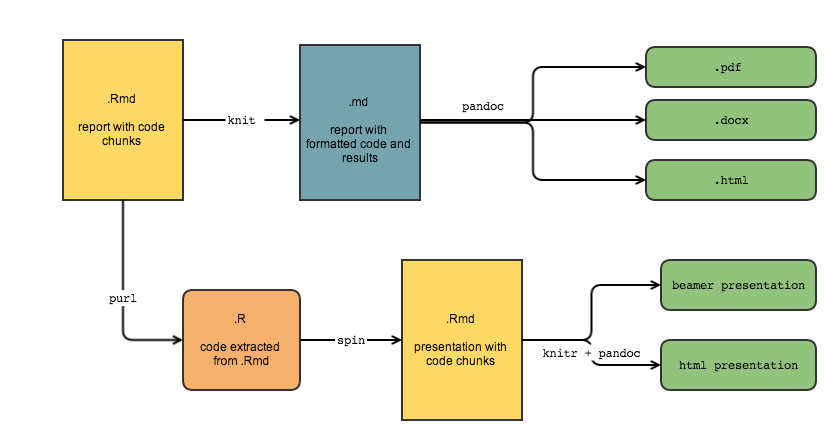
\includegraphics{./figureFiles/knitr-workflow.png}
\end{itemize}

\end{frame}

\subsection{环境安装}

\begin{frame}{环境安装}

\begin{enumerate}
\def\labelenumi{\arabic{enumi}.}
\item
  安装R语言

  \href{https://www.r-project.org/}{Download R}
\item
  安装RStudio

  \href{https://www.rstudio.com/}{Download RStudio}
\item
  安装Texlive

  \href{http://tug.org/texlive/acquire-iso.html}{TeX Live ISO image}
\end{enumerate}

\end{frame}

\section{RMarkdown语法}\label{rmarkdown}

\subsection{文档头定义}

\begin{frame}[fragile]{文档头定义}

\begin{verbatim}
title: R Markdown + Beamer = Perfect Academic Presentation
subtitle:  基于RMarkdown快速制作学术幻灯片
author: Jiangyong Wei
date: '2017-03-05'
fontsize: 10pt
output: 
  beamer_presentation:
    keep_tex: true
    slide_level: 3
    highlight: tango
    pandoc_args: "--latex-engine=xelatex"
    includes:
      in_header: ./texf/header.tex
      before_body: ./texf/prefix.tex
      after_body: ./texf/suffix.tex
    template: ./texf/default_beamer.tex
\end{verbatim}

\end{frame}

\subsection{多级标题}

\begin{frame}[fragile]{多级标题}

\texttt{\#} \(\Rightarrow\) 一级标题section

\vspace{12pt}

\texttt{\#\#} \(\Rightarrow\) 二级标题subsection

\vspace{12pt}

\texttt{\#\#\#} \(\Rightarrow\) 三级标题Frame

\end{frame}

\subsection{字体}

\begin{frame}[fragile]{字体}

\texttt{*字体*} \(\Rightarrow\) \emph{字体}

\vspace{12pt}

\texttt{**字体**} \(\Rightarrow\) \textbf{字体}

\vspace{12pt}

\texttt{\textbackslash{}textcolor\{texpurple\}\{字体\}} \(\Rightarrow\)
\textcolor{texpurple}{字体}

\end{frame}

\subsection{列表}

\begin{frame}[fragile]{有序列表}

\begin{verbatim}
1.  one
2.  two
3.  three
\end{verbatim}

\begin{enumerate}
\def\labelenumi{\arabic{enumi}.}
\tightlist
\item
  one
\item
  two
\item
  three
\end{enumerate}

\end{frame}

\begin{frame}[fragile]{无序列表}

\begin{verbatim}
* fruits
    + apples
        - macintosh
        - red delicious
    + pears
    + peaches
* vegetables
    + broccoli
    + chard
\end{verbatim}

\begin{itemize}
\tightlist
\item
  fruits

  \begin{itemize}
  \tightlist
  \item
    apples

    \begin{itemize}
    \tightlist
    \item
      macintosh
    \item
      red delicious
    \end{itemize}
  \item
    pears
  \item
    peaches
  \end{itemize}
\item
  vegetables

  \begin{itemize}
  \tightlist
  \item
    broccoli
  \item
    chard
  \end{itemize}
\end{itemize}

\end{frame}

\subsection{数学公式}

\begin{frame}[fragile]{数学公式}

\begin{itemize}
\tightlist
\item
  行内公式 \texttt{\$}
\end{itemize}

\texttt{\$\textbackslash{}bf\ ABCDEFG\$} \(\Rightarrow\) \(\bf ABCDEFG\)

\texttt{\$\textbackslash{}rm\ ABCDEFG\$} \(\Rightarrow\) \(\rm ABCDEFG\)

\texttt{\$\textbackslash{}cal\ ABCDEFG\$} \(\Rightarrow\)
\(\cal ABCDEFG\)

\begin{itemize}
\tightlist
\item
  行间公式 \texttt{\$\$}
\end{itemize}

\texttt{\$\$\textbackslash{}begin\{aligned\}\ I(X;Y)\&\ =\ H(X)-H(X\textbar{}Y)\textbackslash{}\textbackslash{}\ \&=\ H(Y)-H(Y\textbar{}X)\textbackslash{}end\{aligned\}\$\$}

\[\begin{aligned} I(X;Y)& = H(X)-H(X|Y)\\
&= H(Y)-H(Y|X)\end{aligned}\]

\end{frame}

\subsection{分栏}

\begin{frame}{分栏}

\begin{columns}[c] % the "c" option specifies center vertical alignment
\column{.5\textwidth} % column designated by a command
Contents of the first column
\column{.5\textwidth}
Contents of the second column
\end{columns}

\end{frame}

\subsection{Block}\label{block}

\begin{frame}{Block}

\begin{itemize}
\tightlist
\item
  block
\end{itemize}

\begin{block}{勾股定理}
  
        直角三角形的斜边的平方等于两直角边的平方和。
可以用符号语言表述为:设直角三角形ABC,其中$\angle C=90^\circ$则有

$$AB^2=BC^2+AC^2$$

\end{block}

\begin{itemize}
\tightlist
\item
  problock
\end{itemize}

\begin{problock}{勾股定理}
  
        直角三角形的斜边的平方等于两直角边的平方和。
可以用符号语言表述为:设直角三角形ABC,其中$\angle C=90^\circ$则有

$$AB^2=BC^2+AC^2$$

\end{problock}

\begin{itemize}
\tightlist
\item
  alertblock \ldots{}
\item
  exampleblock \ldots{}
\end{itemize}

\end{frame}

\subsection{代码}

\begin{frame}[fragile]{代码}

\begin{Shaded}
\begin{Highlighting}[]
\KeywordTok{library}\NormalTok{(knitr)}
\KeywordTok{library}\NormalTok{(rmarkdown)}
\NormalTok{file <-}\StringTok{ }\KeywordTok{list.files}\NormalTok{(}\DataTypeTok{pattern=}\StringTok{'.Rmd'}\NormalTok{)}
\NormalTok{rmarkdown::}\KeywordTok{render}\NormalTok{(file)}
\end{Highlighting}
\end{Shaded}

\end{frame}

\subsection{脚注}

\begin{frame}{脚注}

Here is a footnote reference,\footnote<.->{Here is the footnote.} and
another.\footnote<.->{Here's one with multiple blocks.}

Here is an inline note.\footnote<.->{Inlines notes are easier to write,
  since you don't have to pick an identifier and move down to type the
  note.}

\end{frame}

\subsection{其它}

\begin{frame}{其它}

\begin{itemize}
\tightlist
\item
  表格
\item
  图片
\item
  链接
\item
  引用 \ldots{}
\end{itemize}

\end{frame}

\section{Latex设置}\label{latex}

\subsection{模板设置和中文支持}

\begin{frame}[fragile]{模板设置和中文支持}

\begin{itemize}
\tightlist
\item
  模板设置
\end{itemize}

\begin{verbatim}
    includes:
      in_header: ./texf/header.tex
      before_body: ./texf/prefix.tex
      after_body: ./texf/suffix.tex
    template: ./texf/default_beamer.tex
\end{verbatim}

\begin{itemize}
\tightlist
\item
  中文支持
\end{itemize}

\begin{verbatim}
\usepackage{xeCJK}
\setCJKmainfont{Microsoft YaHei}
\setCJKsansfont{SimHei}
\setCJKmonofont{FangSong}
\end{verbatim}

其它设置请参考in\_header、before\_body、after\_body、template的tex文件定义。

\end{frame}

\begin{frame}[c]{}
 \emph {\Huge{\color{texpurple}\centerline{\CJKfontspec[FakeSlant = 0.2]{STSong}谢谢!} }  }
% \emph {\Huge{\color{texpurple}\centerline{Thank you!} }  }
  \FootText{如有任何意见或建议,请发邮件至首页邮箱。}
% \FootText{\tiny \emph {If you have any comments or suggestions, please contact the email address in the title page.}}

\end{frame}

\end{document}
